\newpage
{\color{secblue}\subsection{Runtime View}}
{\color{secblue}\subsubsection{Registering a new user in TrackMe ecosystem}}
\begin{figure}[H]
    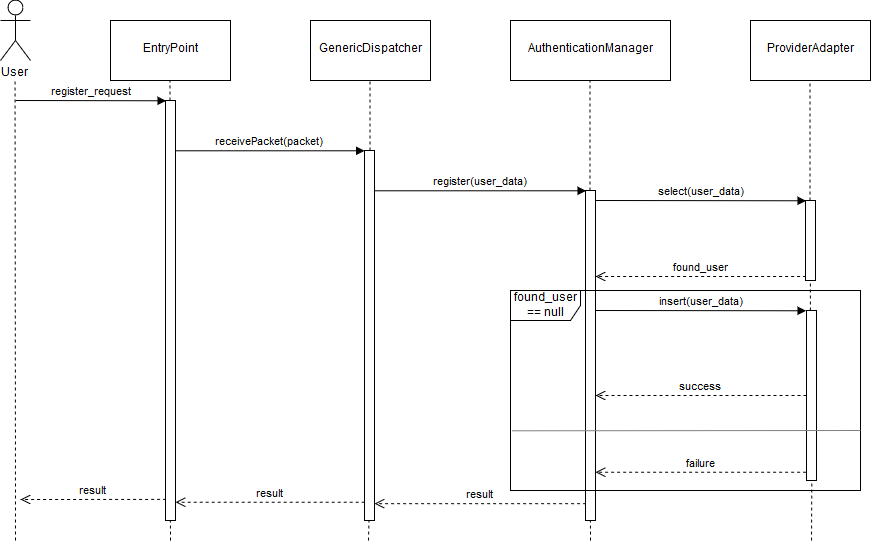
\includegraphics[width=\linewidth, keepaspectratio]{./Images/registering_new_user.png}
    \centering
    \caption{Registering New User}
    \label{fig:depview}
  \end{figure}
This section shows the process of registering a new user. The first thing that happen is that the incoming packet is read by the Entry Point and then passed to the Generic Dispatcher. The Generic Dispatcher reads the type of the packet and forwards it to the Authentication Manager, because no service (D4H, ASOS, nor T4R) is marked in the packet's header. The Authentication Manager finally extrapolate the actual data from the packet and proceed creating a new user: firstly it makes a query to check if the user already exist and if it doesn't it proceed making a query inserting a new user.These two operations are done through the Provider Adapter component.
{\color{secblue}\subsubsection{Storing a new raw data packet in Data4Help}}
\begin{figure}[H]
    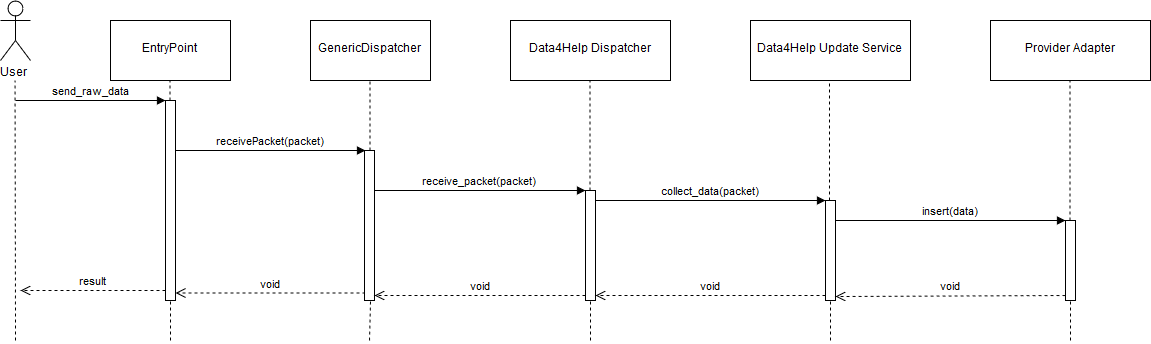
\includegraphics[width=\linewidth, keepaspectratio]{./Images/storing_new_data.png}
    \centering
    \caption{Storing New Data}
    \label{fig:depview}
  \end{figure}
This section shows the process of storing a new raw data packet in the database. The first thing that happen is that the incoming packet is read by the Entry Point and then passed to the Generic Dispatcher. The Generic Dispatcher reads the type of the packet and forwards it to the Data4Help Dispatcher. The Data4Help Dispatcher finally sends it to the D4H Update Service which sends it to the proper services. In this example the only service is Data4Help, so the only component that it is used is the Provider Adapter that make the actual INSERT in the database.
{\color{secblue}\subsubsection{Emergency detected in AutomatedSOS}}
\begin{figure}[H]
    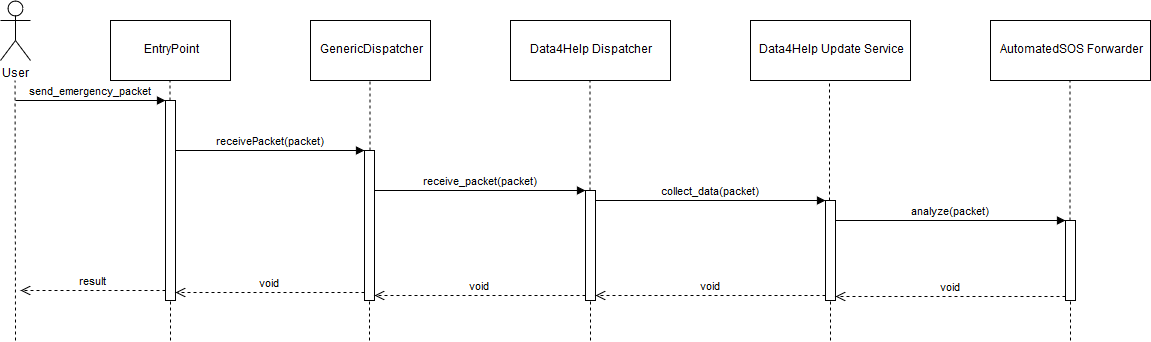
\includegraphics[width=\linewidth, keepaspectratio]{./Images/asos_emergency.png}
    \centering
    \caption{Asos Emergency}
    \label{fig:depview}
  \end{figure}
This section shows the process of detecting an emergency. The first thing that happen is that the incoming packet is read by the Entry Point and then passed to the Generic Dispatcher. The Generic Dispatcher reads the type of the packet and forwards it to the Data4Help Dispatcher. The Data4Help Dispatchersends it to the Data4Help Update Service which finally sends it to the AutomatedSOS Forwarder which is warned that there is an actual emergency and start the procedure for calling the most suitable hospital.
{\color{secblue}\subsubsection{Retrieving the positions of runners in a run in Track4Run}}
\begin{figure}[H]
    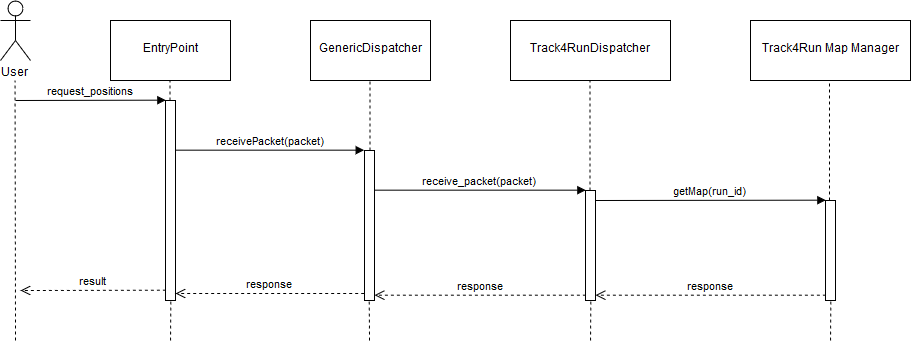
\includegraphics[width=\linewidth, keepaspectratio]{./Images/retrieving_positions.png}
    \centering
    \caption{Retrieving Positions}
    \label{fig:depview}
  \end{figure}
This section shows the process of retrieving the positions of runners in a run. The first thing that happen is that the incoming packet is read by the Entry Point and then passed to the Generic Dispatcher. The Generic Dispatcher reads the type of the packet and forwards it to the Track4Run Dispatcher. The Track4Run Dispatcher finally sends it to the Track4Run Map Manager which packs the data with all the positions of the runners for the specified run and send it back once it is ready.